\section{Ensemble Methods}
\smallskip \hrule height 2pt \smallskip

Vocab
\begin{itemize}
	\item \textbf{decision tree stump}: 
	\item \textbf{decision stub}:  (used in lecture 10 pg 14: boosting)  ?? horizontal or vertical line only?  
	\item \textbf{axis aligned classifier}
\end{itemize}

Instead of learning a single classifier, learn many weak classifiers that are good at different parts of the data. 
The output class is a weighted vote of each classifier. 
\begin{itemize}
	\item classifiers that are most "sure" will vote with more conviction
	\item classifiers will be most "sure" about a particular part of the space. 
	\item on average, these will do better than a single classifier. 
\end{itemize}

% transcribed understanding of audio from week 8
This is better than breaking up the space into a bunch of sub-spaces and making single classifiers for each.  
If you had single classifiers for sub-spaces, you would be losing information about the surroundings.
It is better to have all classifiers cover the whole space, but let them vote. 

\subsection{Bagging}
\textbf{"Bagging" = \underline{B}ootstrap \underline{AGG}regation.}
For $i = 1, 2, \dots, K$:   (?? translate to english ??) 
\begin{itemize}
	\item $T_i \leftarrow$ randomly select $M$ training instances with replacement.
	\item $h_i \leftarrow$ learn($T_i$)
\end{itemize}
Then combine the $h_i$ together with uniform voting ($w_i = 1/K$ for all $i$).

\subsubsection{Example: CART decision boundary}
CART is a decision tree learning algorithm. \hfill \\

100 bagged trees:  shades of blue/red indicate the strength of votes for particular classifications. \hfill \\
Picked random subsets of the data, and built classifiers.  These classifiers are weighted!! \hfill \\  % week 8 audio
?? (not the strength of different classifiers.)   \hfill \\ 
?? Is white an overall uncertain vote ??   \hfill \\ 
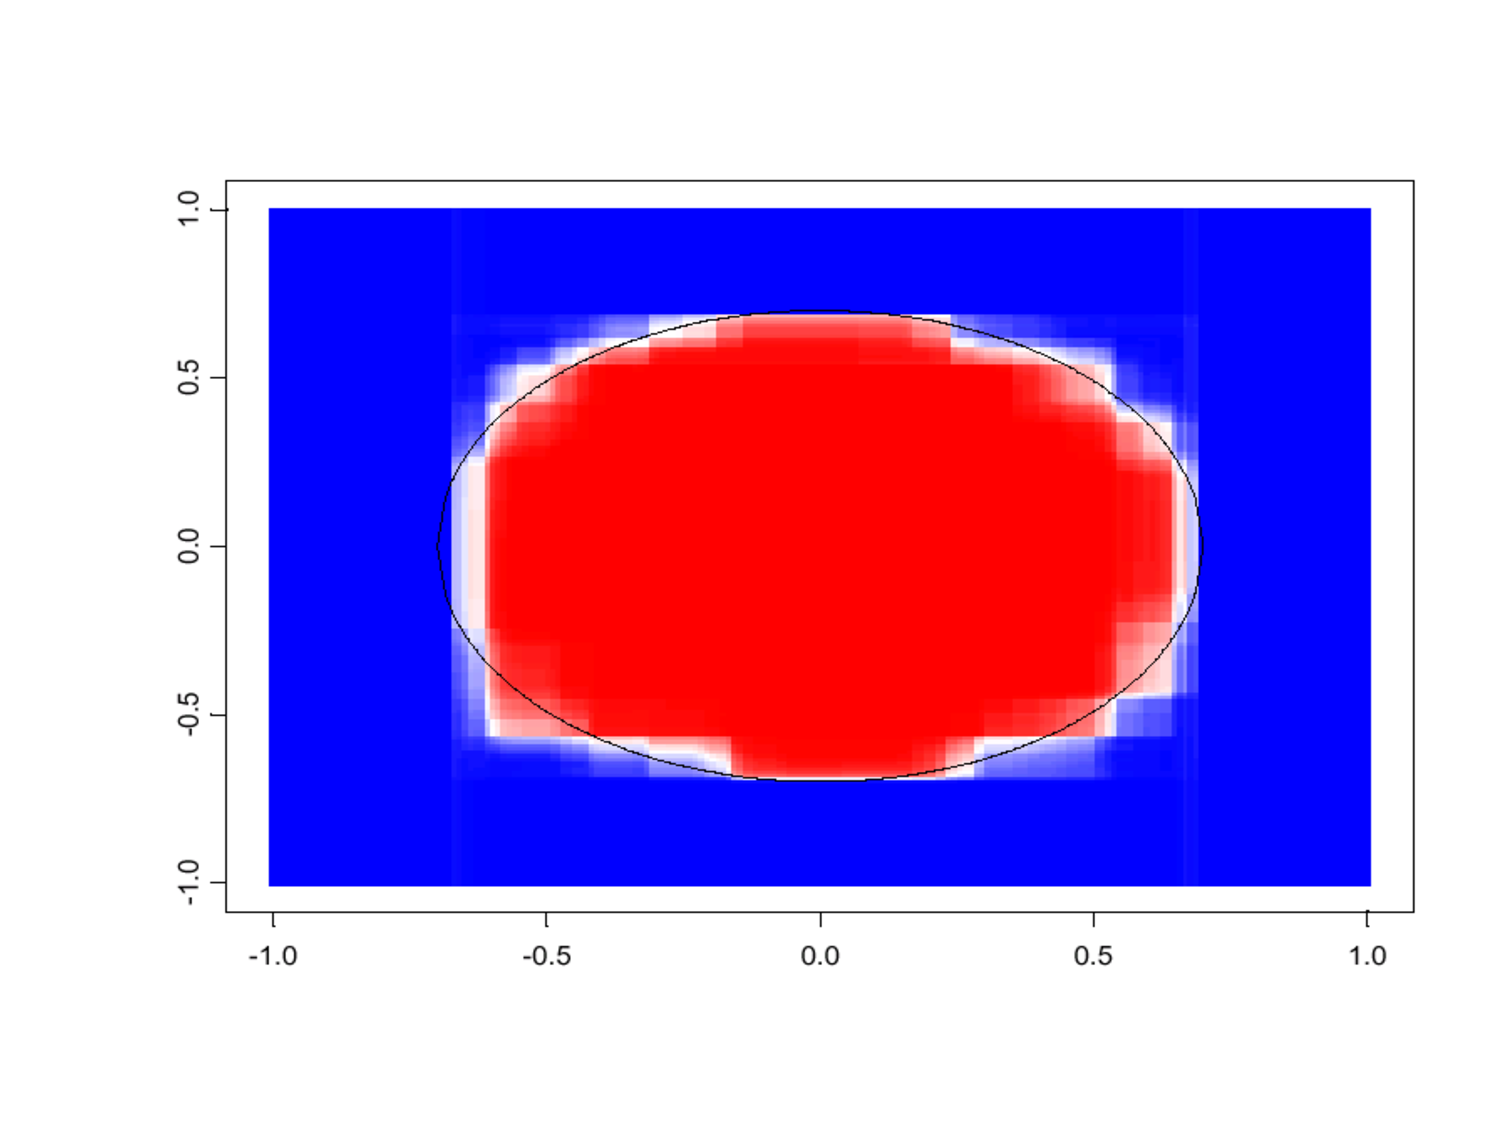
\includegraphics[width=2in]{figures/100_bagged_trees.pdf} \hfill \\
Approximating the circle with a set of lines.  Piecewise linear functions. \hfill \\ % wk 8 audio
The more trees you have, the smoother the boundary will be. 

\subsubsection{Fighting the bias-variance tradeoff}
Simple (a.k.a. weak) learners are good. \hfill \\ 
Examples of weak learners we can use: \hfill \\ 
Naive Bayes, logistic regression, perceptron, decision stumps, shallow decision trees, etc. \hfill \\ 
These learners have low variance; they don't usually overfit. 

But simple (a.k.a. weak) learners are also bad: \hfill \\ 
They have high bias, so you can't solve hard learning problems. \hfill \\ 

The solution: Boosting. 

\subsection{Boosting}
\underline{The idea}: given a weak learner, run it multiple times on (reweighted) training data, 
	then let the learned classifiers vote.  \hfill \\
	
On each iteration $t$:
\begin{itemize}
	\item weight each training example by how incorrectly it was classified.
	\item learn a hypothesis: $h_t$
	\item Use strength $\alpha_t$ for this hypothesis. 
\end{itemize}
Final classifier: $\displaystyle h(x) = sign \left( \sum_i \alpha_i h_i(x)  \right)$ \hfill \\
This is both useful in a practical sense and theoretically interesting. 

Can use boosting with any kind of classifier.  %https://www.youtube.com/watch?v=UHBmv7qCey4

\subsection{Bagging}
Bagging takes a bunch of low bias, high variance functions.
By averaging them, we can reduce the variance without significantly increasing the bias. 

\subsubsection{Learning from weighted data}
Consider a weighted data set: \hfill \\
\begin{itemize}
	\item $D(i)$ is the weight of the $i^{th}$ training example $(\bm{x}^i, \bm{y}^i)$
	\item interpretations:
		\begin{itemize}
			\item $i^{th}$ training example counts as if it occurred $D(i)$ times
			\item if I were to "resample" data, I would get more samples of "heavier" data points. 
		\end{itemize}
	\item Now we always do weighted calculations:
		\begin{itemize}
			\item e.g. MLE for Naive Bayes
			\item redefine Count(Y=y) to be a weighted count: \hfill \\
				$\displaystyle Count(Y=y) = \sum_{j=1}^n D(j) \delta (Y^j = y)$
			\item setting $D(j) = 1$ (or any constant value!) for all $j$ recreates the unweighted case. 
		\end{itemize}
\end{itemize}

